\documentclass[UTF8]{ctexart}
\usepackage[textwidth=444bp,vmargin=2.5cm]{geometry}
%\usepackage{abstract} %生成摘要使用的宏包
\usepackage[colorlinks,linkcolor=black,anchorcolor=black,citecolor=black]{hyperref} %“colorlinks”的意思是将超链接以颜色来标识,而并非使用默认的方框来标识。linkcolor,anchorcolor, citecolor分别表示用来标识link, anchor, cite等各种链接的颜色。此处我们均设为黑色。
\usepackage{fancyhdr} %插入页脚的宏包
\usepackage{graphicx}%图片宏包
\usepackage{float}
\graphicspath{{./figure_pytorch/}}
\DeclareGraphicsExtensions{.pdf,.jpeg,.png,.jpg}%在添加图片后只需要图片的名字,而不需要拓展名
\usepackage{subfigure}%并列插入图片
\usepackage{amsmath}%公式宏包
\usepackage[T1]{fontenc}% 统一修改正文和数学字体为Adobe Utopia, 这个字体和Times有些像
\usepackage{newtxtext, newtxmath}  %两种使用Times New Roman 字体的方法
\linespread{1.5}%设置行间距为1.5倍行距
\renewcommand{\abstractname}{\Large\textbf{摘要}}
\usepackage{appendix}%加入附录需使用appendix宏包
\usepackage{listings}%插入代码
\usepackage{xcolor}

\usepackage{booktabs}
\usepackage{longtable}
\usepackage{array}
\usepackage{multirow}
\usepackage{makecell}
\usepackage{bm}
\usepackage{pythonhighlight}
\usepackage{ctex}
\usepackage[linesnumbered,ruled]{algorithm2e}
\ctexset{
	% 修改 section。
	section={   
		name={,、},
		number={\chinese{section}}
	}
}
\ctexset{
	% 修改 section。
	section={   
		name={,、},
		number={\chinese{section}},
		aftername=\hspace{1pt}
	}
}
\usepackage{enumitem}
\usepackage{tabularx}
%\usepackage{setspace}%使用间距宏包


\begin{document}    %文档的开始,一定要有文档的结束,才能生效
	\setlength{\abovedisplayskip}{2pt}
	\setlength{\belowdisplayskip}{2pt}
	\setlength{\abovedisplayshortskip}{2pt}
	\setlength{\belowdisplayshortskip}{2pt}
	%------------------------标题-------------------------
	%\begin{titlepage}%使页码跳过这页
	\begin{center}
		\heiti\zihao{3}\textbf{3.4 \, softmax回归重点摘录与练习解答} %标题3号加粗
		\vspace{2ex}
	\end{center}
	
	
	%\end{titlepage}
	%-------------------------正文部分-------------------------
	%修改页眉页脚
	\pagestyle{fancy}
	\lhead{}
	\chead{}
	\rhead{}
	%\lfoot{}
	\cfoot{\thepage}
	%\rfoot{} %空格即表示空白
	\renewcommand{\headrulewidth}{0pt}
	\renewcommand{\footrulewidth}{0pt} %设置页眉页脚分割线的宽度,如果为0pt,则不显示线条
	
	\textbf{(1)独热编码}
	
	但一般的分类问题并不与类别之间的自然顺序有关。统计学家很早以前就发明了一种表示分类数据的简单方法:独热编码(one-hot encoding)。独热编码是一个向量,它的分量和类别一样多。类别对应的分量设置为 1,其他所有分量设置为 0。在我们的例子中,标签 $\bm{y}$ 将是一个三维向量,其中 $(1, 0, 0)$ 对应于“猫”、$(0, 1, 0)$ 对应于“鸡”、$(0, 0, 1)$ 对应于“狗”:
	$$
	\bm{y} \in \{(1, 0, 0), (0, 1, 0), (0, 0, 1)\}.
	$$
	
	\textbf{(2)网络构架}
	
	与线性回归一样,softmax 回归也是一个单层神经网络,由于计算每个输出 $o_1$、$o_2$ 和 $o_3$ 取决于所有输入 $\bm{x}_1$、$\bm{x}_2$、$\bm{x}_3$ 和 $\bm{x}_4$,所以softmax回归的输出层也是全连接层。
	\begin{figure}[H]
		\centering
		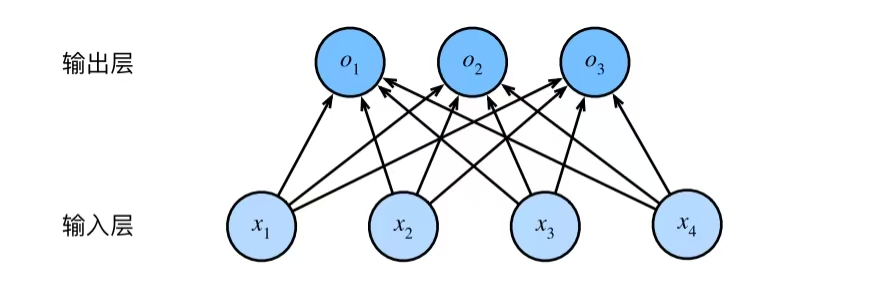
\includegraphics[width=0.6\textwidth]{3.4_1}
		\caption{单层神经网络}
		\label{fig:1}
	\end{figure}
	
	\textbf{(3)Softmax 运算}
	
	现在我们将优化参数以最大化观测数据的概率。为了得到预测结果,我们将设置一个阈值,如选择具有最大概率的标签。
	
	我们希望模型的输出 $\hat{\bm{y}}_j$ 可以视为属于类 $j$ 的概率,然后选择具有最大输出值的类别 $\arg \max_j \hat{\bm{y}}_j$ 作为我们的预测。例如,如果 $\hat{\bm{y}}_1$、$\hat{\bm{y}}_2$ 和 $\hat{\bm{y}}_3$ 分别为 0.1、0.8 和 0.1,那么我们预测的类别是 2,在我们的例子中代表“鸡”。
	
	然而我们不能直接将未规范化的预测 $o$ 直接视作我们感兴趣的输出,因为在通常情况下,
	\[
	\sum_i o_i \neq 1,
	\]
	并且由于输入的不同,可能存在 $o_i< 0$ 的情况,直接作为概率是不适合的。
	
	因此使用 softmax 函数对概率进行校正:softmax 函数能够将未规范化的预测变换为非负数并且总和为1,同时让模型保持可导的性质。
	$$
	\hat{\bm{y}} = softmax(\bm{o}) \quad \text{其中} \quad \hat{\bm{y}}_j =  \frac{\exp(o_j)}{\displaystyle\sum_k \exp(o_k)}
	$$
	这里,对于所有的 $j$ 总有 $0 \leq \hat{\bm{y}}_j \leq 1$。因此,$\hat{\bm{y}}$ 可以视为一个正确的概率分布。softmax运算不会改变未规范化的预测 $\bm{o}$ 之间的大小次序,只会确定分配给每个类别的概率。因此,在预测过程中,我们仍然可以用下式来选择最有可能的类别。
	$$
	\arg \max_j \hat{\bm{y}}_j = \arg \max_j o_j.
	$$
	
	尽管 softmax 函数是一个非线性函数,但 softmax 回归的输出仍然由输入特征的仿射变换决定,故 softmax 回归是一个线性模型(linear model)。
	
	\textbf{(4)小批量样本的矢量化}
	
	假设我们读取了一个批量的样本 $\bm{X}$,其中特征维度(输入数量)为 $d$,批量大小为 $n$。此外,假设我们在输出中有 $q$ 个类别。那么小批量样本的特征为 $\bm{X} \in \mathbb{R}^{n \times d}$,权重为 $\bm{W} \in \mathbb{R}^{d \times q}$,偏置为 $\bm{b} \in \mathbb{R}^{1 \times q}$。softmax 回归的矢量计算表达式为:
	$$
	\bm{O} = \bm{X} \bm{W} + \bm{b},
	$$
	$$
	\hat{\bm{Y}} = softmax(\bm{O}).
	$$
	
	\textbf{(5)损失函数的相关推导}
	
	softmax函数给出了一个向量 $\hat{\bm{y}}$,我们可以将其视为“对给定任意输入 $\bm{x}$ 的每个类的条件概率”。假设整个数据集 $\bm{X}, \bm{Y}$ 具有 $n$ 个样本,其中索引 $i$ 的样本由特征向量 $\bm{x}^{(i)}$ 和独热标签向量 $\bm{y}^{(i)}$ 组成。根据独立性写出似然函数如下:
	\[
	L(\bm{Y} \mid \bm{X}) = \prod_{i=1}^n P(\bm{y}^{(i)} \mid \bm{x}^{(i)}).
	\]
	
	根据 MLE ,我们最大化 $L(\bm{Y} \mid \bm{X})$,相当于最小化负对数似然:
	\[
	\arg \min \left( -\log L(\bm{Y} \mid \bm{X})\right) 
	= \arg \min \left( - \sum_{i=1}^n \log P(\bm{y}^{(i)} \mid \bm{x}^{(i)}) \right) 
	= \arg \min \sum_{i=1}^n l(\bm{y}^{(i)}, \hat{\bm{y}}^{(i)}) ,
	\]
	其中,对于任何标签 $\bm{y}$ 和模型预测 $\hat{\bm{y}}$,使用交叉熵(cross-entropy)损失函数:
	\[
	l(\bm{y}, \hat{\bm{y}}) = -\sum_{j=1}^q y_j \log \hat{y}_j .
	\]
	由于 $\bm{y}$ 是一个长度为 $q$ 的独热编码向量,则:
	\[
	y_i=
	\begin{cases}
		1,\; i=j,\\
		0,\; i \neq j.
	\end{cases}
	\]
	由于所有 $\hat{y}_j$ 都是预测的概率,所以它们的对数永远不会大于 0。
	
	下面是对于交叉熵损失函数的推导:对于第 $i$ 行,$ l(\bm{y}^{(i)}, \hat{\bm{y}}^{(i)}) = -\log P(\bm{y}^{(i)} \mid \bm{x}^{(i)}) $,其中,$P(\bm{y}^{(i)} \mid \bm{x}^{(i)})$ 意为给定 $\bm{x}^{(i)}$ 时,$\bm{y}^{(i)}$ 的条件概率,且 $\bm{y}^{(i)}$ 的 $q$ 个项中,
	\[
	y_j=1, \;and \;  y_i=0,\forall i \neq j.
	\]
	因此有:
	\[
	\sum_{j=1}^q \bm{y}_j \log \hat{\bm{y}}_j = 0 \times \log \hat{\bm{y}}_1 + \cdots + 1 \times \log \hat{\bm{y}}_j + \cdots + 0 \times \log \hat{\bm{y}}_q= \log \hat{\bm{y}}_j
	\]
	根据条件概率的性质可知有:$ P(\bm{y}^{(i)} \mid \bm{x}^{(i)}) = \frac{\exp(o_j)}{\sum_{k=1}^q \exp(o_k)} = \hat{\bm{y}}_j$. 因此:
	\[
	l(\bm{y}^{(i)}, \hat{\bm{y}}^{(i)}) = -\log P(\bm{y}^{(i)} \mid \bm{x}^{(i)}) = -\log \hat{\bm{y}}_j = -\sum_{j=1}^q \bm{y}_j \log \hat{\bm{y}}_j
	\]
	
	\textbf{(6)softmax 及其导数}
	
	由于softmax和相关的损失函数很常见,因此我们需要更好地理解它的计算方式。利用softmax的定义,$\sum_{j=1}^q y_j=1$我们得到:
	\begin{eqnarray*}
		l(\bm{y}, \hat{\bm{y}}) &=& -\sum_{j=1}^q y_j \log \frac{\exp(o_j)}{\sum_{k=1}^q \exp(o_k)}\\
		&=& \sum_{j=1}^q y_j \log \sum_{k=1}^q \exp(o_k) - \sum_{j=1}^q y_j o_j\\
		&=& \left(\log \sum_{k=1}^q \exp(o_k) \right) \cdot \left( \sum_{j=1}^q y_j\right) - \sum_{j=1}^q y_j o_j\\
		&=& \log \sum_{k=1}^q \exp(o_k) - \sum_{j=1}^q y_j o_j.
	\end{eqnarray*}
	
	
	考虑相对于任何未规范化的预测 $o_j$ 的导数,我们得到:
	\[
	\partial_{o_j} l(\bm{y}, \hat{\bm{y}}) = \frac{\exp(o_j)}{\sum_{k=1}^q \exp(o_k)} - y_j = \text{softmax}(\bm{o})_j - y_j.
	\]
	
	换句话说,导数是我们softmax模型分配的概率与实际发生的情况(由独热标签向量表示)之间的差异。从这个意义上讲,这与我们在回归中看到的非常相似,其中梯度是观测值 $\bm{y}$ 和估计值 $\hat{\bm{y}}$ 之间的差。
	
	\newpage
	\textbf{(7)问题解答}
	
	\textbf{1、我们可以更深入地探讨指数族与softmax之间的联系}
	
	\noindent \textbf{解}:计算softmax交叉熵损失 $ l(\bm{y}, \hat{\bm{y}}) $ 的二阶导数:
		$$
		\partial_{o_j} l(\bm{y}, \hat{\bm{y}}) = \frac{\exp(o_j)}{\sum_{k=1}^q \exp(o_k)} - y_j = \text{softmax}(\bm{o})_j - y_j
		$$
		
		\begin{eqnarray*}
			\partial_{o_j}^2 l(\bm{y}, \hat{\bm{y}}) &=& \frac{\exp(o_j) \sum_{k=1}^q \exp(o_k) - \exp(o_j)^2}{\left( \sum_{k=1}^q \exp(o_k) \right)^2}\\
			&=& softmax(\bm{o})_j - softmax(\bm{o})_j^2\\
			&=& softmax(\bm{o})_j (1 - softmax(\bm{o})_j)
		\end{eqnarray*}
	
	计算 $\text{softmax}(\bm{o})$ 给出的分布方差,并与上面计算的二阶导数匹配,期望计算如下:
	\begin{eqnarray*}
		E[softmax(\bm{o})_j] &=& \frac{1}{q} \sum_{j=1}^q 1 \cdot softmax(\bm{o})_j \\
		&=& \frac{1}{q} \sum_{j=1}^q \frac{\exp(o_j)}{\sum_k \exp(o_k)} \\
		&=& \frac{1}{q}.
	\end{eqnarray*}
	
	方差计算如下:
	\begin{eqnarray*}
		Var[\bm{o}] &=& E[(softmax(\bm{o})_j - E[softmax(\bm{o})_j])^2]\\
		&=& \frac{1}{q} \sum_{j=1}^q (softmax(\bm{o})_j - \frac{1}{q})^2\\
		&=& \frac{1}{q} \left[ \sum_{j=1}^q softmax^2(\bm{o})_j - \frac{2}{q} \sum_{j=1}^q softmax(\bm{o})_j + \frac{1}{q} \right]\\
		&=& -\frac{1}{q} \left[ \sum_{j=1}^q softmax(\bm{o})_j - \sum_{j=1}^q softmax^2(\bm{o})_j + \frac{2}{q} - 1 - \frac{1}{q} \right]\\
		&=& \frac{q-1}{q^2} - \frac{1}{q} \sum_{j=1}^q (softmax(\bm{o})_j - softmax^2(\bm{o})_j)\\
		&=& \frac{q-1}{q^2} - \frac{1}{q} \sum_{j=1}^q \partial_{o_j}^2 l(\bm{y}, \hat{\bm{y}}).
	\end{eqnarray*}
	
	
	\newpage
	\textbf{3、softmax 是对上面介绍的映射的误称(虽然深度学习领域中很多人都使用这个名字)。真正的 softmax 被定义为  $RealSoftMax(a, b) = \log(e^a + e^b)$。}
	
	\noindent \textbf{解}:首先证明 $\text{RealSoftMax}(a, b) > \max(a, b)$。
	
	不妨假设假设 $\max(a, b) = a$,则
	\begin{eqnarray*}
		RealSoftMax(a, b) &=& \log(e^a + e^b) \\
		&>& \log(e^a)  \\
		&=& a =\max(a, b).
	\end{eqnarray*}
	
	然后证明 $\frac{1}{\lambda} RealSoftMax(\lambda a, \lambda b) > \max(a, b)$ 成立,前提是 $\lambda > 0$,
	
	则当 $\lambda > 0$ 时,假设 $\max(a, b) = a$
	\begin{eqnarray*}
		\frac{1}{\lambda} \text{RealSoftMax}(\lambda a, \lambda b) &=& \frac{1}{\lambda} \log(e^{\lambda a} + e^{\lambda b}) \\
		&>& \frac{1}{\lambda} \log(e^{\lambda a})  \\
		&=&a=  \max(a, b).
	\end{eqnarray*}
	
	然后证明对于 $\lambda \to \infty$,有 $\displaystyle \lim_{\lambda \to \infty}\frac{1}{\lambda} RealSoftMax(\lambda a, \lambda b) = \max(a, b)$;
	
	不妨设 $\max(a, b) = a$,则有:
	\[
	e^{\lambda a} < e^{\lambda a} + e^{\lambda b} < 2\cdot e^{\lambda a}
	\]
	
	因此有
	\begin{eqnarray*}
		a &=&  \lim_{\lambda \to \infty}\frac{ \log (e^{\lambda a})}{\lambda} \\
		& \leqslant & \lim_{\lambda \to \infty}\frac{\log (e^{\lambda a} + e^{\lambda b})}{\lambda}  \\ 
		&=&\lim_{\lambda \to \infty}\frac{1}{\lambda} RealSoftMax(\lambda a, \lambda b)\\
		& \leqslant & \lim_{\lambda \to \infty}\frac{\log (2\cdot e^{\lambda a} )}{\lambda}  \\
		&=& \lim_{\lambda \to \infty}\frac{\log 2}{\lambda}   + \lim_{\lambda \to \infty}\frac{\log (e^{\lambda a} )}{\lambda}  \\
		&=& a.
	\end{eqnarray*}
	
	由夹逼原理可知结论成立。
	
	而soft-min表达式如下:
	$$
	\text{softmin}(\bm{o}) _j= \frac{\exp(-o_j)}{\sum_k \exp(-o_k)}
	$$
	

	%正文中引用到参考文献的地方\cite{01} \cite{02}
	%-------------------------附录部分-------------------------
	% 使用\begin{appendices} \end{appendices} 或者直接用\appendix
	\appendix
	%代码格式设置,代码的设置与具体的编程语言有关,比赛时上网搜素即可
	\definecolor{dkgreen}{rgb}{0,0.6,0}
	\definecolor{gray}{rgb}{0.5,0.5,0.5}
	\definecolor{mauve}{rgb}{0.58,0,0.82}
	\definecolor{mydarkblue}{RGB}{0, 0, 128} % 示例:深蓝色,RGB值为(0, 0, 128) 
	\definecolor{codegreen}{rgb}{0,0.6,0}
	\definecolor{codegray}{rgb}{0.5,0.5,0.5}
	\definecolor{codepurple}{rgb}{0.58,0,0.82}
	\definecolor{backcolour}{rgb}{0.95,0.95,0.92}
	\lstset{ %
		language=Python,                % the language of the code
		basicstyle=\footnotesize,           % the size of the fonts that are used for the code
		numbers=left,                   % where to put the line-numbers
		numberstyle=\tiny\color{gray},  % the style that is used for the line-numbers
		stepnumber=2,                   % the step between two line-numbers. If it's 1, each line 
		% will be numbered
		numbersep=5pt,                  % how far the line-numbers are from the code
		backgroundcolor=\color{white},      % choose the background color. You must add \usepackage{color}
		showspaces=false,               % show spaces adding particular underscores
		showstringspaces=false,         % underline spaces within strings
		showtabs=false,                 % show tabs within strings adding particular underscores
		frame=single,                   % adds a frame around the code
		rulecolor=\color{black},        % if not set, the frame-color may be changed on line-breaks within not-black text (e.g. commens (green here))
		tabsize=2,                      % sets default tabsize to 2 spaces
		captionpos=b,                   % sets the caption-position to bottom
		breaklines=true,                % sets automatic line breaking
		breakatwhitespace=false,        % sets if automatic breaks should only happen at whitespace
		title=\lstname,                   % show the filename of files included with \lstinputlisting;
		% also try caption instead of title
		keywordstyle=\color{blue},          % keyword style
		commentstyle=\color{codegreen},       % comment style
		stringstyle=\color{codepurple},         % string literal style
		escapeinside={\%*}{*)},            % if you want to add LaTeX within your code
		morekeywords={*,...}               % if you want to add more keywords to the set
	}

	
	\end{document}